\documentclass[11pt,a4paper]{article}

\usepackage[margin=1in]{geometry}
\usepackage{amsmath,amssymb,amsthm}
\usepackage{graphicx}
\usepackage{booktabs}
\usepackage{enumitem}
\usepackage{hyperref}
\usepackage{xcolor}
\usepackage{listings}
\usepackage{algorithm}
\usepackage{algorithmic}
\usepackage{tcolorbox}
\usepackage{fancyhdr}
\usepackage{multicol}
\usepackage{fontawesome5}
\usepackage{pifont}

\tcbuselibrary{breakable,skins}

% Theorem environments
\theoremstyle{definition}
\newtheorem{definition}{Definition}[section]
\newtheorem{example}{Example}[section]
\newtheorem{remark}{Remark}[section]
\theoremstyle{plain}
\newtheorem{proposition}{Proposition}[section]

% Custom boxes
\newtcolorbox{keytakeaway}{colback=green!5!white,colframe=green!50!black,title={Key Takeaway},fonttitle=\bfseries,breakable}
\newtcolorbox{pitfall}{colback=red!5!white,colframe=red!60!black,title={Common Pitfall},fonttitle=\bfseries,breakable}
\newtcolorbox{production}{colback=blue!5!white,colframe=blue!50!black,title={Production Note},fonttitle=\bfseries,breakable}

% Code listings
\lstset{language=Python,basicstyle=\ttfamily\footnotesize,keywordstyle=\color{blue},commentstyle=\color{gray},stringstyle=\color{red},showstringspaces=false,breaklines=true,frame=single,numbers=left,numberstyle=\tiny\color{gray},backgroundcolor=\color{gray!10},xleftmargin=2em,framexleftmargin=1.5em}

% TikZ libraries for included figures
\usetikzlibrary{shapes,arrows,positioning,calc,patterns,decorations.pathreplacing,shadows,fit}

% Header/Footer
\pagestyle{fancy}
\fancyhf{}
\fancyhead[L]{\textsc{Information Retrieval}}
\fancyhead[R]{\textsc{Lecture 1: Introduction \& Vector Space Model}}
\fancyfoot[C]{\thepage}

\title{\textbf{Lecture 1: Introduction \& Vector Space Model}\\[0.5em]\Large Information Retrieval --- Lecture Notes}
\author{Avishek Anand\\\textit{Information Retrieval Course}}
\date{\today}

% Custom macros and TikZ styles
\usepackage{tikz}
\usetikzlibrary{positioning, shapes, arrows, shadows, fit, calc, decorations.pathreplacing}

% Semantic Colors - One meaning per color
\definecolor{irSparse}{HTML}{3498DB}   % Sparse/BM25: Blue
\definecolor{irDense}{HTML}{E67E22}    % Dense/Embeddings: Orange
\definecolor{irRerank}{HTML}{C0392B}   % Rerank/Cross-encoder: Red
\definecolor{irHybrid}{HTML}{2ECC71}   % Hybrid/Fusion: Green
\definecolor{irANN}{HTML}{9B59B6}      % ANN/Infra: Purple
\definecolor{irInfra}{HTML}{58595B}    % General Infra: Dark Gray
\definecolor{irMuted}{HTML}{D9D9D9}    % Faint Gray

% Base Styles - Consistent Diagram Grammar
\tikzset{
    irBoxBase/.style={
        rectangle, 
        draw, 
        rounded corners=2pt, 
        minimum height=0.8cm, 
        minimum width=2cm,
        font=\small\sffamily,
        align=center,
        drop shadow={opacity=0.15},
        inner sep=5pt
    },
    irDatabase/.style={
        cylinder, 
        draw, 
        shape border rotate=90, 
        aspect=0.25, 
        minimum height=1.2cm, 
        minimum width=1cm,
        fill=irMuted!20,
        draw=irInfra,
        font=\tiny\sffamily,
        align=center
    },
    % Semantic Variants
    sparse/.style={irBoxBase, fill=irSparse!10, draw=irSparse},
    dense/.style={irBoxBase, fill=irDense!10, draw=irDense},
    rerank/.style={irBoxBase, fill=irRerank!10, draw=irRerank},
    hybrid/.style={irBoxBase, fill=irHybrid!10, draw=irHybrid},
    ann/.style={irBoxBase, fill=irANN!10, draw=irANN},
    infra/.style={irBoxBase, fill=irInfra!10, draw=irInfra},
    % Legacy support / Utility
    muted/.style={irBoxBase, fill=irMuted!20, draw=irMuted!80!black, text=irMuted!50!black},
    ghost/.style={irBoxBase, fill=white, draw=irMuted!50, text=irMuted, dashed, drop shadow={opacity=0}},
    emph/.style={draw=irRerank, thick, drop shadow={shadow xshift=0mm, shadow yshift=0mm, fill=irRerank, opacity=0.3}},
    % Arrows
    irArrowBase/.style={->, thick, >=latex, draw=irInfra},
    irLabel/.style={
        font=\tiny\itshape, 
        text=irInfra, 
        align=center, 
        text width=2.5cm, 
        inner sep=3pt
    }
}


% =========================================================
% Stage Badge System
% =========================================================
% \irStage{StageName}
\newcommand{\irStage}[1]{%
    \begin{tikzpicture}[remember picture, overlay]
        \node[
            anchor=north east,
            fill=irInfra!10,
            text=irInfra,
            font=\tiny\bfseries,
            inner sep=3pt,
            rounded corners=1pt,
            yshift=-0.5cm,
            xshift=-0.5cm
        ] at (current page.north east) {#1};
    \end{tikzpicture}%
}

% =========================================================
% Math Highlighting
% =========================================================
% \mathhl[color]{content}
\newcommand{\mathhl}[2][irDense!30]{%
    \colorbox{#1}{$\displaystyle #2$}%
}

% =========================================================
% Math Vectors
% =========================================================
\newcommand{\vs}{\mathbf{s}}

% =========================================================
% Core Box Primitives
% =========================================================
% \IRBox[width]{id}{at}{title}{subtitle}{variant}
% Default width chosen for lecture slides; override when needed.
% \IRBox[width]{id}{at}{title}{subtitle}{variant}[extra options]
\DeclareDocumentCommand{\IRBox}{O{3.5cm} m m m m m O{}}{%
    \node[#6, text width=#1, #7] (#2) at #3 {%
        \textbf{#4}%
        \if\relax\detokenize{#5}\relax
        \else\\[-1mm]\scriptsize #5%
        \fi
    };%
}

% \IRWideBox{id}{at}{width}{title}{subtitle}{variant}
\newcommand{\IRWideBox}[6]{%
    \node[#6, text width=#3] (#1) at #2 {%
        \textbf{#4}%
        \if\relax\detokenize{#5}\relax
        \else\\[-1mm]\scriptsize #5%
        \fi
    };%
}

% =========================================================
% Arrow Primitives
% =========================================================
% Safe default: left-to-right flow
% \IRArrow{from}{to}{label}
\newcommand{\IRArrow}[3]{%
    \draw[irArrowBase] (#1.east) -- node[irArrowLabelAbove] {#3} (#2.west);%
}

% Explicit left-to-right
% \IRArrowLR{from}{to}{label}
\newcommand{\IRArrowLR}[3]{%
    \draw[irArrowBase] (#1.east) -- node[irArrowLabelAbove] {#3} (#2.west);%
}

% Explicit top-to-bottom
% \IRArrowTB{from}{to}{label}
\newcommand{\IRArrowTB}[3]{%
    \draw[irArrowBase] (#1.south) -- node[irArrowLabelRight] {#3} (#2.north);%
}

% Fully explicit anchor-to-anchor path
% \IRArrowPath{from anchor}{to anchor}{label}
% Example: \IRArrowPath{a.east}{b.north}{score}
\newcommand{\IRArrowPath}[3]{%
    \draw[irArrowBase] (#1) -- node[irArrowLabelAbove] {#3} (#2);%
}

% Orthogonal elbow path
% \IRArrowElbow{from anchor}{to anchor}{label}
% Example: \IRArrowElbow{a.east}{b.north}{feedback}
\newcommand{\IRArrowElbow}[3]{%
    \draw[irArrowBase] (#1) -| node[irArrowLabelBox] {#3} (#2);%
}

% Slanted arrow for special cases only
% \IRArrowSlanted{from anchor}{to anchor}{label}{pos}{width}
\newcommand{\IRArrowSlanted}[5]{%
    \draw[irArrowBase] (#1) -- node[above, sloped, irLabel, pos=#4, text width=#5, fill=white, inner sep=1pt] {#3} (#2);%
}

% =========================================================
% Accent Elements
% =========================================================
% \IRBadge{at}{text}
\newcommand{\IRBadge}[2]{%
    \node[
        draw=irAccent,
        fill=irAccent!20,
        rounded corners=1pt,
        font=\tiny\bfseries,
        inner sep=2pt
    ] at #1 {#2};%
}

% =========================================================
% Grouping
% =========================================================
% \IRGroup{fit nodes}{label}{variant}
% Example: \IRGroup{(a)(b)(c)}{First-stage retrieval}{muted}
\newcommand{\IRGroup}[3]{%
    \node[
        irGroupBase,
        #3,
        fit=#1
    ] (group) {};
    \node[
        anchor=north west,
        font=\tiny\bfseries,
        #3
    ] at ([xshift=2pt,yshift=-2pt] group.north west) {#2};%
}

% =========================================================
% Domain-Specific Shapes
% =========================================================
% \IRDocStack{id}{at}{label}
\newcommand{\IRDocStack}[3]{%
    \node[irDocStack] (#1) at #2 {#3};%
}

% \IRDatabase{id}{at}{label}
\newcommand{\IRDatabase}[3]{%
    \node[irDatabase] (#1) at #2 {#3};%
}

% =========================================================
% Layout Helpers
% =========================================================
% \IRPipelineTier{id}{at}{text}{label}{variant}
\newcommand{\IRPipelineTier}[5]{%
    \IRBox{#1}{#2}{#3}{}{#5}[]
    \node[anchor=west, irLabel, xshift=0.5cm] at (#1.east) {#4};%
}

% \IRTelescopeTier{id}{at}{width}{text}{variant}
\newcommand{\IRTelescopeTier}[5]{%
    \node[
        irTelescopeBase,
        #5,
        minimum width=#3
    ] (#1) at #2 {#4};%
}

% \IRStep{id}{at}{title}{subtitle}{variant}
% Creates a numbered step badge left of a box.
\newcommand{\IRStep}[5]{%
    \node[
        circle,
        draw=irAccent,
        fill=irAccent!20,
        font=\tiny\bfseries,
        inner sep=2pt
    ] (#1_num) at #2 {#1};
    \node[
        #5,
        text width=3.5cm,
        right=1.5cm of #1_num
    ] (#1) {%
        \textbf{#3}%
        \if\relax\detokenize{#4}\relax
        \else\\[-1mm]\scriptsize #4%
        \fi
    };
    \draw[irArrowBase, thin] (#1_num.east) -- (#1.west);%
}


\begin{document}
\maketitle

\begin{abstract}
These lecture notes accompany Lecture~1 of the Information Retrieval course. We introduce the fundamental concepts of Information Retrieval (IR), distinguishing it from database systems and natural language processing. We explore the core challenges of scale and semantic understanding before diving into the two classical retrieval models: the \textbf{Boolean Retrieval Model} and the \textbf{Vector Space Model (VSM)}. Key topics include TF-IDF term weighting and cosine similarity.
\end{abstract}

\tableofcontents
\newpage

%=======================================================================
\section{What is Information Retrieval?}
\label{sec:what-is-ir}
%=======================================================================

\begin{definition}[Information Retrieval]
Information Retrieval (IR) is the field concerned with finding material (usually documents) of an unstructured nature (usually text) that satisfies an information need within large collections.
\end{definition}

In essence, IR is about bridging the gap between a user's \emph{information need} and a massive collection of items. Unlike structured data retrieval in databases, IR deals with the inherent ambiguity of natural language.

\subsection{IR vs. Database Systems}

The primary difference between IR and Database Management Systems (DBMS) lies in the structure of the data and the precision of the query.

\begin{center}
\begin{tabular}{lll}
\toprule
\textbf{Aspect} & \textbf{Database Systems} & \textbf{IR Systems} \\
\midrule
Data & Structured (tables, schemas) & Unstructured (text, documents) \\
Queries & Precise (SQL) & Vague (natural language) \\
Matching & Exact & Approximate/Ranked \\
Result & All matching records & Top-$k$ relevant documents \\
Failure & No results or all results & Ranked list (best effort) \\
\bottomrule
\end{tabular}
\end{center}

\begin{keytakeaway}
Databases ask: \textit{``Give me all records matching X''}. IR asks: \textit{``Give me the most relevant documents about X''}.
\end{keytakeaway}

\subsection{IR vs. Natural Language Processing (NLP)}

While IR and NLP share tools (like tokenizers and embeddings), they have different focal points:
\begin{itemize}
    \item \textbf{NLP (Understanding):} Focuses on language representation, syntax, semantics, and generation.
    \item \textbf{IR (Retrieval):} Focuses on information seeking, scale, and ranking.
\end{itemize}

%=======================================================================
\section{The Core Challenges of IR}
\label{sec:challenges}
%=======================================================================

\subsection{The Semantic Gap}

The most significant challenge in IR is the \emph{semantic gap}---the difference between the keywords used in a query and the underlying intent of the user.

\begin{center}
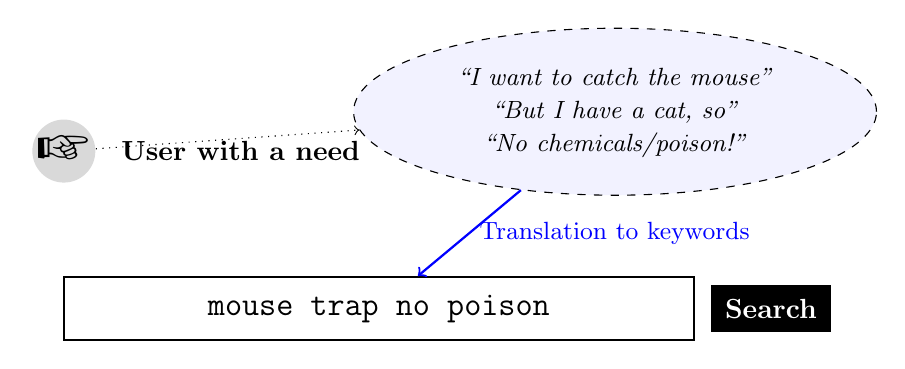
\begin{tikzpicture}[
    searchbox/.style={rectangle, draw, thick, minimum width=8cm, minimum height=0.8cm, font=\large},
    user/.style={circle, fill=gray!30, minimum size=0.8cm},
    icon/.style={font=\huge}
]
    % User Icon
    \node[user] (u) at (0,3) {};
    \node[icon] at (u) {\ding{43}}; % Hand/User representation
    \node[right=0.2cm of u] {\textbf{User with a need}};

    % Search Box
    \node[searchbox, fill=white] (box) at (4,1) {\texttt{mouse trap no poison}};
    \node[right=0.2cm of box, fill=black, text=white, inner sep=5pt] {\textbf{Search}};
    
    % Cloud / Intent
    \node[draw, ellipse, dashed, fill=blue!5, minimum width=4cm, minimum height=1.5cm] (intent) at (7,3.5) {
        \begin{tabular}{c}
            \small \textit{``I want to catch the mouse''} \\
            \small \textit{``But I have a cat, so''} \\
            \small \textit{``No chemicals/poison!''}
        \end{tabular}
    };
    \draw[->, dotted] (u) -- (intent);
    \draw[->, thick, blue] (intent) -- (box) node[midway, right] {\small Translation to keywords};
\end{tikzpicture}

\end{center}

For a query like \texttt{mouse trap no poison}, a simple keyword matching system might return documents discussing how poison traps work because the words ``poison'' and ``trap'' appear. However, the user's intent is to find \emph{mechanical} or \emph{humane} alternatives.

\subsection{Scale and Freshness}

Modern IR systems must operate at a scale that is difficult to comprehend:
\begin{itemize}
    \item \textbf{Scale:} Google indexes over 100 trillion pages.
    \item \textbf{Throughput:} Billions of queries per day.
    \item \textbf{Latency:} Sub-second response times are mandatory.
    \item \textbf{Freshness:} The index must reflect the state of the web in near real-time.
\end{itemize}

%=======================================================================
\section{The Information Retrieval Problem}
\label{sec:ir-problem}
%=======================================================================

The retrieval process follows a cycle where a user formulates a need into a query, the system searches a collection, and the user evaluates the ranked results.

\begin{center}
\begin{tikzpicture}[
    scale=0.45, transform shape,
    node distance=1.8cm,
    box/.style={rectangle, draw, rounded corners=2pt, fill=blue!10, text width=4cm, align=center, minimum height=0.8cm, font=\small},
    arrow/.style={->, thick, -{Stealth[length=2.2mm]}}
]
    \node[box, fill=irInfra!10] (user) {User Information Need};
    \node[box, below=of user] (query) {Query Formulation\\(Text String)};
    \node[box, below=of query] (system) {Search Engine Logic};
    \node[box, below=of system] (collection) {Document Index};
    \node[box, below=of collection] (results) {Ranked Results List};
    \node[box, below=of results, fill=irAccent!10] (satisfy) {User Satisfaction};

    \draw[arrow] (user.south) -- (query.north) node[midway, right, font=\tiny] {formulate};
    \draw[arrow] (query.south) -- (system.north) node[midway, right, font=\tiny] {submit};
    \draw[arrow] (system.south) -- (collection.north) node[midway, right, font=\tiny] {index lookup};
    \draw[arrow] (collection.south) -- (results.north) node[midway, right, font=\tiny] {rank};
    \draw[arrow] (results.south) -- (satisfy.north) node[midway, right, font=\tiny] {evaluate};

    % Optional backlink
    \draw[arrow, dashed, irMuted] (satisfy.west) .. controls +(-1.5,0) and +(-1.5,0) .. (user.west) 
        node[midway, left, font=\tiny, rotate=90] {reformulate};

\end{tikzpicture}

\end{center}

This process raises three fundamental questions that define the design of any IR system:
\begin{enumerate}
    \item How do we represent documents and queries?
    \item How do we match queries to documents efficiently?
    \item How do we rank documents by relevance?
\end{enumerate}

%=======================================================================
\section{The Boolean Retrieval Model}
\label{sec:boolean}
%=======================================================================

The Boolean model is the simplest retrieval model. It treats documents as sets of terms and queries as Boolean expressions.

\begin{definition}[Boolean Retrieval]
In the \emph{Boolean retrieval model}, a document is retrieved if it satisfies a Boolean expression of query terms using operators \texttt{AND}, \texttt{OR}, and \texttt{NOT}.
\end{definition}

\subsection{Query Processing with Set Operations}

Queries are processed as set intersections, unions, and differences of posting lists (the sets of document IDs containing each term).

\begin{example}[Boolean Query Tree]
Consider the query: \texttt{(cat AND mat) OR dog}. The system first intersects the sets of documents containing ``cat'' and ``mat'', then unions the result with the set of documents containing ``dog''.

\begin{center}
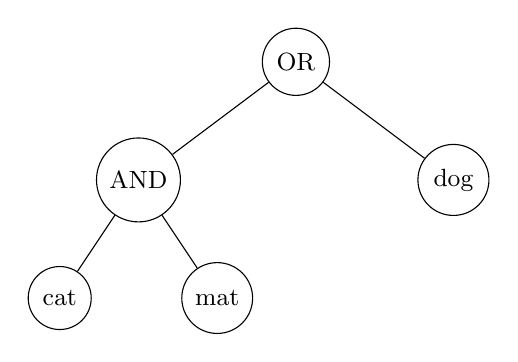
\begin{tikzpicture}[
    level distance=1.5cm,
    level 1/.style={sibling distance=4cm},
    level 2/.style={sibling distance=2cm},
    every node/.style={circle, draw, minimum size=0.8cm, font=\small}
]
    \node {OR}
        child {node {AND}
            child {node {cat}}
            child {node {mat}}
        }
        child {node {dog}};
\end{tikzpicture}

\end{center}
\end{example}

\subsection{The Feast or Famine Problem}

Boolean retrieval suffers from a binary view of relevance: a document is either in or out.
\begin{itemize}
    \item \textbf{Famine:} A query with too many \texttt{AND} terms may return 0 results if even one minor term is missing (too restrictive).
    \item \textbf{Feast:} A broad query may return millions of results with no way to identify the best ones (too permissive).
\end{itemize}

\begin{keytakeaway}
Boolean retrieval lacks \textbf{ranking} and \textbf{partial matching}. This motivates the transition to weighted models like the Vector Space Model.
\end{keytakeaway}

%=======================================================================
\section{The Vector Space Model (VSM)}
\label{sec:vsm}
%=======================================================================

The Vector Space Model represents documents and queries as vectors in a high-dimensional space, where each dimension corresponds to a term in the vocabulary.

\begin{center}
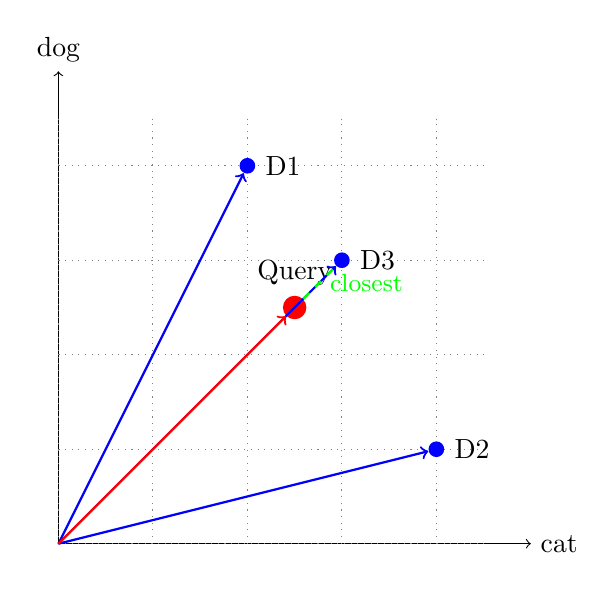
\begin{tikzpicture}[scale=1.2]
    % Axes
    \draw[->] (0,0) -- (5,0) node[right] {cat};
    \draw[->] (0,0) -- (0,5) node[above] {dog};
    
    % Grid
    \draw[gray, dotted] (0,0) grid (4.5,4.5);
    
    % Documents
    \node[circle, fill=blue, inner sep=2pt, label=right:D1] (d1) at (2,4) {};
    \node[circle, fill=blue, inner sep=2pt, label=right:D2] (d2) at (4,1) {};
    \node[circle, fill=blue, inner sep=2pt, label=right:D3] (d3) at (3,3) {};
    
    % Query
    \node[circle, fill=red, inner sep=3pt, label=above:Query] (q) at (2.5,2.5) {};
    
    % Vectors
    \draw[->, thick, blue] (0,0) -- (d1);
    \draw[->, thick, blue] (0,0) -- (d2);
    \draw[->, thick, blue] (0,0) -- (d3);
    \draw[->, thick, red] (0,0) -- (q);
    
    % Similarity illustration
    \draw[dashed, green, thick] (q) -- (d3) node[midway, right] {\small closest};
\end{tikzpicture}

\end{center}

\subsection{Term Weighting: TF-IDF}

To create meaningful vectors, we must assign weights to terms. The standard approach is \textbf{TF-IDF} (Term Frequency-Inverse Document Frequency).

\begin{definition}[TF-IDF]
The weight of term $t$ in document $d$ is:
\[ w_{t,d} = \mathrm{tf}(t,d) \times \log\left(\frac{N}{\mathrm{df}(t)}\right) \]
where:
\begin{itemize}
    \item $\mathrm{tf}(t,d)$ is the number of occurrences of term $t$ in document $d$.
    \item $N$ is the total number of documents in the collection.
    \item $\mathrm{df}(t)$ is the number of documents containing term $t$.
\end{itemize}
\end{definition}

\textbf{Intuition:}
\begin{itemize}
    \item \textbf{TF} rewards terms that appear often in a document (local importance).
    \item \textbf{IDF} penalizes terms that appear often in the collection (stop words like ``the'') and rewards rare, discriminative terms (global importance).
\end{itemize}

\subsection{Worked Example: TF-IDF Calculation}

\begin{example}[TF-IDF Weights]
Collection of 10,000 documents. Document $d$ contains: ``neural'' (5 times), ``network'' (3 times), and ``the'' (50 times).
\begin{center}
\begin{tabular}{lcccc}
\toprule
\textbf{Term} & \textbf{tf(t,d)} & \textbf{df(t)} & \textbf{idf(t)} & \textbf{tf-idf} \\
\midrule
neural & 5 & 100 & $\log(10000/100) = 2.0$ & 10.0 \\
network & 3 & 500 & $\log(10000/500) = 1.3$ & 3.9 \\
the & 50 & 9000 & $\log(10000/9000) = 0.05$ & 2.5 \\
\bottomrule
\end{tabular}
\end{center}
Despite appearing 10 times more often, ``the'' receives a lower weight than ``neural'' because it carries less discriminative information.
\end{example}

%=======================================================================
\section{Cosine Similarity}
\label{sec:cosine}
%=======================================================================

In VSM, the relevance of a document to a query is measured by the \emph{cosine} of the angle between their vectors.

\begin{definition}[Cosine Similarity]
The similarity between query vector $\vec{q}$ and document vector $\vec{d}$ is:
\[ \mathrm{sim}(\vec{q}, \vec{d}) = \frac{\vec{q} \cdot \vec{d}}{\|\vec{q}\| \|\vec{d}\|} = \frac{\sum_{t} q_t \times d_t}{\sqrt{\sum_{t} q_t^2} \times \sqrt{\sum_{t} d_t^2}} \]
\end{definition}

\begin{keytakeaway}
Cosine similarity normalizes for document length. Without this normalization, long documents would naturally have larger dot products simply because they contain more words, regardless of their actual relevance.
\end{keytakeaway}

%=======================================================================
\section{VSM vs. Boolean Retrieval}
\label{sec:comparison}
%=======================================================================

\begin{center}
\begin{tabular}{lll}
\toprule
\textbf{Aspect} & \textbf{Boolean} & \textbf{Vector Space} \\
\midrule
Matching & Exact (in/out) & Partial (weighted) \\
Ranking & No & Yes (by similarity) \\
Robustness & Brittle & Graceful degradation \\
Term weighting & Binary & TF-IDF \\
User friendliness & Expert users & General users \\
\bottomrule
\end{tabular}
\end{center}

\begin{remark}[Bag of Words Assumption]
Both Boolean and simple VSM models share the \textbf{bag-of-words} assumption: they treat documents as unordered collections of words, ignoring grammar and word order. This limitation is addressed in later lectures using phrase matching and transformer-based models.
\end{remark}

\end{document}
